% ------------------------------------------------------------------------------
% Este fichero es parte de la plantilla LaTeX para la realización de Proyectos
% Final de Grado, protegido bajo los términos de la licencia GFDL.
% Para más información, la licencia completa viene incluida en el
% fichero fdl-1.3.tex

% Copyright (C) 2012 SPI-FM. Universidad de Cádiz
% ------------------------------------------------------------------------------


\section{Metodología de desarrollo}
El modelo de ciclo de vida empleado en el desarrollo del proyecto es el modelo incremental. Este modelo combina elementos del modelo lineal secuencial aplicado repetidamente conjunto a la filosofía de contrucción de prototipos.\\
Cuando se utiliza el modelo incremental en el primer incremento se afrontan requisitos básicos pero muchas funciones suplementarias quedan sin extraer. Como resultado del primer incremento se produce el producto central, el cual posteriormente de la utilización y/o evaluación se modifica a fin de cumplir todos los requisitos y necesidades del cliente.\\

\section{Planificación del proyecto}
La planificación temporal estimada que se ha llevado a cabo durante el desarrollo del proyecto es el siguiente:\\
\begin{itemize}
\item \textbf{Fase de Inicio (18/05/11 - 15/06/11)}: Durante esta etapa se plantea la idea y se consulta con los tutores si es adecuada y la disponibilidad.\\
\item \textbf{Fase de Desarrollo (16/06/11 - 09/08/12)}: Durante esta etapa se desarrolla el proyecto.
\begin{itemize}
\item \textbf{Especificación de requisitos (16/06/11 - 29/07/11)}: La toma de requisitos fue una labor compleja, debido a los constantes cambios y añadidos de funcionalidades. Finalmente se determinaron con éxito todas las funcionalidades y exigencias para el proyecto.
\item \textbf{Análisis (01/08/11 - 12/10/11)}: Teniendo los requisitos bien definidos el análisis ha sido más claro aunque también duradero.
\item \textbf{Diseño (13/10/11 - 30/01/12)}: Así como la implementación, ambas han sido las etapas que más tiempo han consumido. Esta etapa se ha hecho con especial cuidado de realizar un diseño correcto para no interrumpir la implementación por posibles errores.
\item \textbf{Implementación (30/01/12 - 12/07/12)}: Dicha etapa ha sido la más larga durante el desarrollo, en la que se han implementado todos los requisitos satisfaciendo las necesidades previstas.
\item \textbf{Pruebas (13/07/12 - 09/08/12)}: Se han probado todas las funcionalidades comprobando su correcto funcionamiento y ejecución, asegurándose que no hay ningún tipo de error.
\end{itemize}
\item \textbf{Fase de Documentación (10/08/12 - 03/12/12)}: En esta etapa se redactó este documento y todos los necesarios para el complemento del proyecto.
\end{itemize}

Esta planificación se observa mejor en el siguiente diagrama de Gantt.\\
Para mayor legibilidad del diagrama de Gantt, se omite en éste las entregas del producto esencial (o primer incremento), así como sus posteriores incrementos\\
Para realizar el diagrama de ``Gantt'', se ha utilizado la herramienta \textit{Gantt Project}.\\

\begin{figure}[H]
  \label{finicio}
  \begin{center}
    % Comentar si no está el paquete tkiz instalado, y descomentar la
    % linea siguiente. Comentar además la inclusión del paquete en
    % estilos/estiloBase.sty
    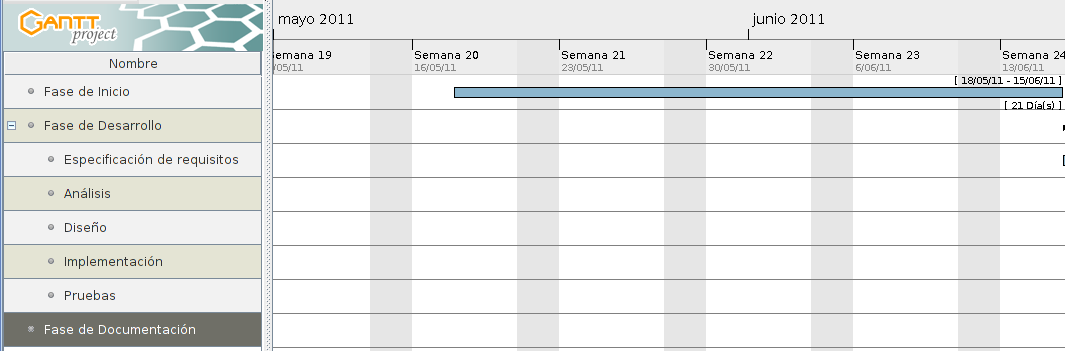
\includegraphics[scale=0.4]{../img/fase-inicio.png} 
  \end{center}
  \caption{Diagrama de Gantt: Fase de Inicio}
\end{figure}

\begin{figure}[H]
  \label{fdes}
  \begin{center}
    % Comentar si no está el paquete tkiz instalado, y descomentar la
    % linea siguiente. Comentar además la inclusión del paquete en
    % estilos/estiloBase.sty
    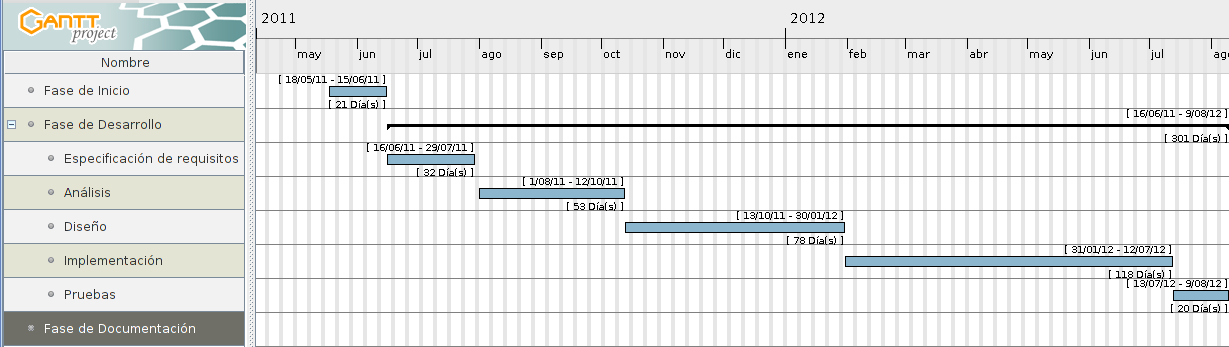
\includegraphics[scale=0.4]{../img/fase-desarrollo.png} 
  \end{center}
  \caption{Diagrama de Gantt: Fase de Desarrollo}
\end{figure}

\begin{figure}[H]
  \label{fdoc}
  \begin{center}
    % Comentar si no está el paquete tkiz instalado, y descomentar la
    % linea siguiente. Comentar además la inclusión del paquete en
    % estilos/estiloBase.sty
    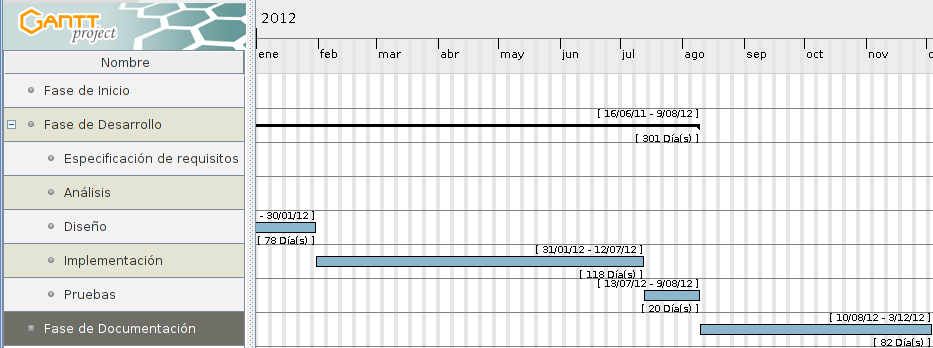
\includegraphics[scale=0.5]{../img/fase-documentacion.png} 
  \end{center}
  \caption{Diagrama de Gantt: Fase de Documentación}
\end{figure}